\documentclass{article}

% Language setting
% Replace `english' with e.g. `spanish' to change the document language
\usepackage[english]{babel}

% Set page size and margins
% Replace `letterpaper' with `a4paper' for UK/EU standard size
\usepackage[letterpaper,top=2cm,bottom=2cm,left=3cm,right=3cm,marginparwidth=1.75cm]{geometry}

% Useful packages
\usepackage{amsmath}
\usepackage{graphicx}
\usepackage{mathbbol}
\usepackage{amsthm}
\usepackage{amssymb}
\usepackage[colorlinks=true, allcolors=blue]{hyperref}
\usepackage{listings}

% Font size
\usepackage{setspace}
\doublespacing

% tree
\usepackage{tikz}

\title{CSCB63 Assignment 1}
\author{Zheyuan Wei}

\begin{document}
\maketitle

\section*{Q1}

\subsection*{Q1-a}


\text{Q: }
$ If\ f(n) \in \mathcal{O}(g)\ and\ g \in \mathcal{O}(h)\ then\ f \in \mathcal{O}(h), for\ all\ f, g, h \ in\ \mathbb{N} \rightarrow \mathbb{R^+} $

\begin{proof}

    \text{\newline}

    $ \text{1) From } f \in \text{O(g)} \ we\ have: $
    $$ \exists c_1, n_1 \in \mathbb{R} \text{ s.t. } f(n) \leq c_1 \cdot g(n) \forall n \geq n_1 $$

    $ \text{2) From } g \in \text{O(h)} \ we\ have: $
    $$ \exists c_2, n_2 \in \mathbb{R} \text{ s.t. } g(n) \leq c_2 \cdot h(n) \forall n \geq n_2 $$

    $ \text{3) From 1) \ and\ 2) \ we\ have: }$
    $$ f(x)=\left\{
        \begin{aligned}
            f(n) \leq c_1 \cdot g(n) \forall n \geq n_0, & \text{for some $c_1$ and $n_1$} \\
            g(n) \leq c_2 \cdot h(n) \forall n \geq n_1, & \text{for some $c_2$ and $n_2$} \\
        \end{aligned}
        \right.\\
        \Rightarrow
        \begin{aligned}
            f(n) \leq c_1 ( c_2 \cdot h(n) ) \forall s.t.
            \left\{
            \begin{aligned}
                n \geq n_1 \\
                n \geq n_2 \\
            \end{aligned}
            \right.
        \end{aligned}
    $$
    $ \text{4) From 3) \ we\ have: }$
    $$ f(n) \leq c_1 \cdot c_2 \cdot h(n)\ \forall n \geq max(n_1, n_2) $$
    $$ \Rightarrow f \in \mathcal{O}(h) $$
    % $$ \blacksquare $$

\end{proof}

\newpage

\subsection*{Q1-b}

\text{Q: }
$ If\ f \in \Omega(g)\ and\ g \in \Omega(h)\ then\ f \in \Omega(h), for\ all\ f, g, h\ in\ \mathbb{N} \rightarrow \mathbb{R^+} $

\begin{proof}

    \text{\newline}

    $ \text{1) From} \ f \in \Omega(g) \ \text{we have: } $
    $$ \exists c_1, n_1 \in \mathbb{R} \text{ s.t. } f(n) \geq c_1 \cdot g(n) \forall n \geq n_1 $$

    $ \text{2) From} \ g \in \Omega(h) \ \text{we have: } $
    $$ \exists c_2, n_2 \in \mathbb{R} \text{ s.t. } g(n) \geq c_2 \cdot h(n) \forall n \geq n_2 $$

    $ \text{3) From 1) \ and\ 2) \ we\ have: }$
    $$ f(x)=\left\{
        \begin{aligned}
            f(n) \geq c_1 \cdot g(n) \forall n \geq n_0, & \text{for some $c_1$ and $n_1$} \\
            g(n) \geq c_2 \cdot h(n) \forall n \geq n_1, & \text{for some $c_2$ and $n_2$} \\
        \end{aligned}
        \right.\\
        \Rightarrow
        \begin{aligned}
            f(n) \geq c_1 ( c_2 \cdot h(n) ) \forall s.t.
            \left\{
            \begin{aligned}
                n \geq n_0 \\
                n \geq n_1 \\
            \end{aligned}
            \right.
        \end{aligned}
    $$

    $ \text{4) From 3) \ we\ have: }$
    $$ f(n) \geq c_1 \cdot c_2 \cdot h(n)\ \forall n \geq max(n_0, n_1) $$
    $$ \Rightarrow f \in \Omega(h) $$
    % $$ \blacksquare $$

\end{proof}

\newpage

\subsection*{Q1-c}
\text{Q: \\}
$ \log_\phi(\sqrt{5}(n+2)) - 2 \in \mathcal{O}(\log_2(n)) $
$ \text{where} \ \phi \text{ is the golden ratio.} $

\begin{proof}

    $ \text{Let } f(n) = \log_\phi(\sqrt{5}(n+2)) - 2, \forall n \geq 0 $

    $ \text{Then it follows that: } $

    $$ f(n) = \log_\phi(\sqrt{5}(n+2)) - 2 = \frac{\log_2(\sqrt{5}(n+2))}{\log_2(\phi)} - 2 $$
    $$ f(n) = \frac{\log_\phi{\sqrt{5}}}{\log_2(\phi)} \cdot \log_2(n+2) - 2 $$
    $$ f(n) < \frac{\log_\phi{\sqrt{5}}}{\log_2(\phi)} \cdot \log_2(n+2) = k \cdot \log_2(n+2) \ \forall n \geq 0 $$
    $ \text{where } k = \frac{\log_\phi{\sqrt{5}}}{\log_2(\phi)} \in \mathbb{R} $
    $$ \Rightarrow f(n) < k \cdot \log_2(n+2) \leq k \cdot \log_2(n^2) = k \cdot 2 \cdot \log_2(n) \ \forall n \geq 2 $$
    $ \text{which is equivalent to: } $
    $$ f(n) < 2k \cdot \log_2(n) \ \forall n \geq 2 $$
    $$ \Rightarrow f(n) \in \mathcal{O}(\log_2(n)) $$
    % $$ \blacksquare $$
\end{proof}

\newpage

\section*{Q2}

\subsection*{Q2-a}

\text{Q: }
\text{On an initially empty tree, show each step of inserting the keys 9, 10, 12, 14, 3, 34, 19, 37, 20. }

\paragraph{Step 1: Insert 9 \\}
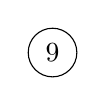
\begin{tikzpicture}[every node/.style={draw,circle,minimum size=3ex}]
    \node (root) {9};
\end{tikzpicture}

\paragraph{Step 2: Insert 10 \\}
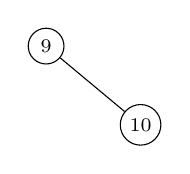
\begin{tikzpicture}[%level distance=5mm,
        level 1/.style={level distance=10mm,sibling distance=24mm},
        level 2/.style={level distance=10mm,sibling distance=16mm},
        level 3/.style={level distance=8mm,sibling distance=8mm},
        font=\scriptsize,inner sep=2pt,every node/.style={draw,circle,minimum size=3ex}]

    \node {9}
    child [missing]
    child   {node {10}}; % right child
\end{tikzpicture}

\paragraph{Step 3: Insert 12 \\}
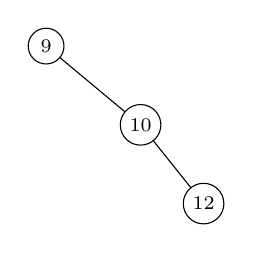
\begin{tikzpicture}[%level distance=5mm,
        level 1/.style={level distance=10mm,sibling distance=24mm},
        level 2/.style={level distance=10mm,sibling distance=16mm},
        level 3/.style={level distance=8mm,sibling distance=8mm},
        font=\scriptsize,inner sep=2pt,every node/.style={draw,circle,minimum size=3ex}]

    \node {9}
    child [missing] % left child
    child   {node {10} % right child
            child [missing] % level 2
            child   {node {12}}};
\end{tikzpicture}
\\
Imbalanced. Right heavy at node 9. \\
Need a left rotation. \\
Left rotation: \\\\
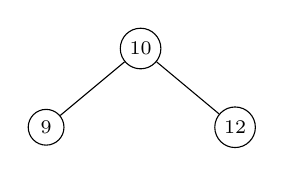
\begin{tikzpicture}[%level distance=5mm,
        level 1/.style={level distance=10mm,sibling distance=24mm},
        level 2/.style={level distance=10mm,sibling distance=16mm},
        level 3/.style={level distance=8mm,sibling distance=8mm},
        font=\scriptsize,inner sep=2pt,every node/.style={draw,circle,minimum size=3ex}]

    \node {10}
    child   {node {9}}
    child   {node {12}};
\end{tikzpicture}

\paragraph{Step 4: Insert 14 \\}
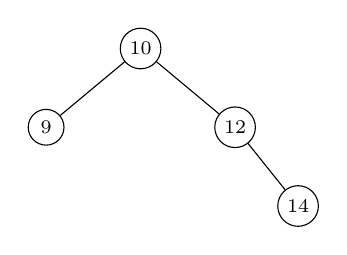
\begin{tikzpicture}[%level distance=5mm,
        level 1/.style={level distance=10mm,sibling distance=24mm},
        level 2/.style={level distance=10mm,sibling distance=16mm},
        level 3/.style={level distance=8mm,sibling distance=8mm},
        font=\scriptsize,inner sep=2pt,every node/.style={draw,circle,minimum size=3ex}]

    \node {10}
    child   {node {9}}
    child   {node {12}
            child [missing]
            child   {node {14}}};
\end{tikzpicture}

\paragraph{Step 5: Insert 3 \\}
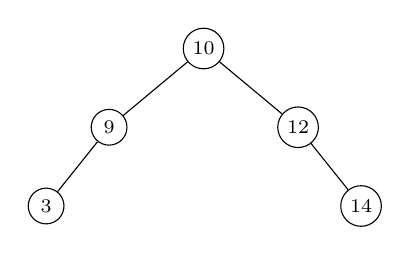
\begin{tikzpicture}[%level distance=5mm,
        level 1/.style={level distance=10mm,sibling distance=24mm},
        level 2/.style={level distance=10mm,sibling distance=16mm},
        level 3/.style={level distance=8mm,sibling distance=8mm},
        font=\scriptsize,inner sep=2pt,every node/.style={draw,circle,minimum size=3ex}]

    \node {10}
    child   {node {9}
            child   {node {3}}
            child [missing]}
    child   {node {12}
            child [missing]
            child   {node {14}}};
\end{tikzpicture}

\paragraph{Step 6: Insert 34 \\}
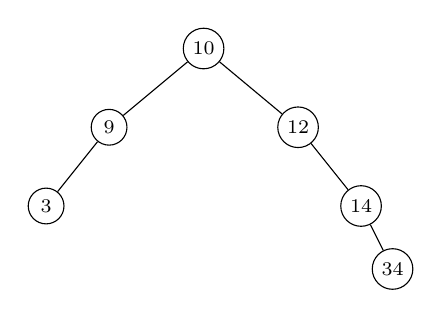
\begin{tikzpicture}[%level distance=5mm,
        level 1/.style={level distance=10mm,sibling distance=24mm},
        level 2/.style={level distance=10mm,sibling distance=16mm},
        level 3/.style={level distance=8mm,sibling distance=8mm},
        level 4/.style={level distance=8mm,sibling distance=4mm},
        font=\scriptsize,inner sep=2pt,every node/.style={draw,circle,minimum size=3ex}]

    \node {10}
    child   {node {9}
            child   {node {3}}
            child [missing]}
    child   {node {12}
            child [missing]
            child   {node {14}
                    child [missing]
                    child   {node {34}}}};
\end{tikzpicture}
\\
Imbalanced. Right heavy at node 12. \\
Need a left rotation. \\
Left rotation: \\\\
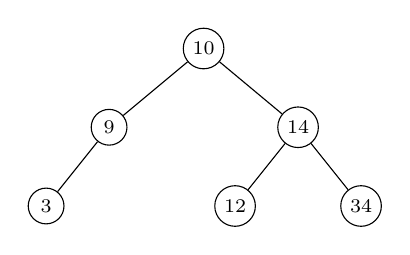
\begin{tikzpicture}[%level distance=5mm,
        level 1/.style={level distance=10mm,sibling distance=24mm},
        level 2/.style={level distance=10mm,sibling distance=16mm},
        level 3/.style={level distance=8mm,sibling distance=8mm},
        font=\scriptsize,inner sep=2pt,every node/.style={draw,circle,minimum size=3ex}]

    \node {10}
    child   {node {9}
            child   {node {3}}
            child [missing]}
    child   {node {14}
            child   {node {12}}
            child   {node {34}}};
\end{tikzpicture}

\paragraph{Step 7: Insert 19 \\}
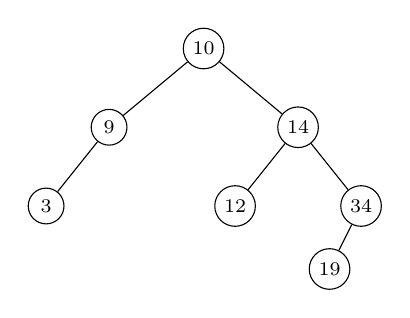
\begin{tikzpicture}[%level distance=5mm,
        level 1/.style={level distance=10mm,sibling distance=24mm},
        level 2/.style={level distance=10mm,sibling distance=16mm},
        level 3/.style={level distance=8mm,sibling distance=8mm},
        level 4/.style={level distance=8mm,sibling distance=4mm},
        font=\scriptsize,inner sep=2pt,every node/.style={draw,circle,minimum size=3ex}]

    \node {10}
    child   {node {9}
            child   {node {3}}
            child [missing]}
    child   {node {14}
            child   {node {12}}
            child   {node {34}
                    child   {node {19}}
                    child [missing]}};
\end{tikzpicture}

\paragraph{Step 8: Insert 37 \\}
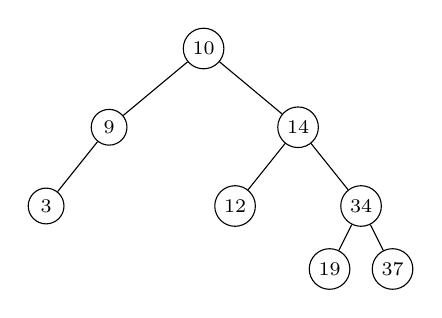
\begin{tikzpicture}[%level distance=5mm,
        level 1/.style={level distance=10mm,sibling distance=24mm},
        level 2/.style={level distance=10mm,sibling distance=16mm},
        level 3/.style={level distance=8mm,sibling distance=8mm},
        level 4/.style={level distance=8mm,sibling distance=4mm},
        font=\scriptsize,inner sep=2pt,every node/.style={draw,circle,minimum size=3ex}]

    \node {10}
    child   {node {9}
            child   {node {3}}
            child [missing]}
    child   {node {14}
            child   {node {12}}
            child   {node {34}
                    child   {node {19}}
                    child   {node {37}}}};
\end{tikzpicture}

\paragraph{Step 9: Insert 20 \\}
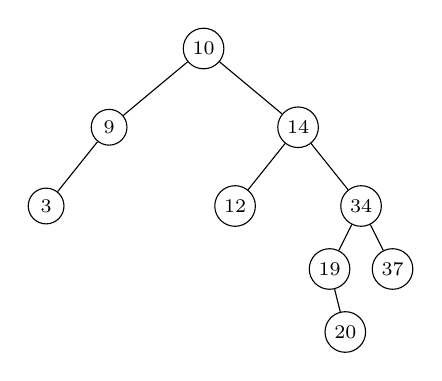
\begin{tikzpicture}[%level distance=5mm,
        level 1/.style={level distance=10mm,sibling distance=24mm},
        level 2/.style={level distance=10mm,sibling distance=16mm},
        level 3/.style={level distance=8mm,sibling distance=8mm},
        level 4/.style={level distance=8mm,sibling distance=4mm},
        font=\scriptsize,inner sep=2pt,every node/.style={draw,circle,minimum size=3ex}]

    \node {10}
    child   {node {9}
            child   {node {3}}
            child [missing]}
    child   {node {14}
            child   {node {12}}
            child   {node {34}
                    child   {node {19}
                            child [missing]
                            child   {node {20}}}
                    child   {node {37}}}};
\end{tikzpicture}
\\
Imbalanced. Right heavy at node 14. \\
Need a double rotation. \\
1. Right rotation: \\\\
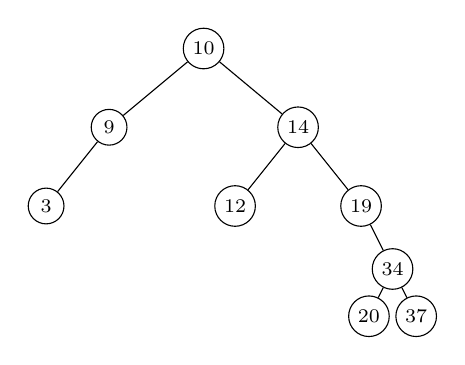
\begin{tikzpicture}[%level distance=5mm,
        level 1/.style={level distance=10mm,sibling distance=24mm},
        level 2/.style={level distance=10mm,sibling distance=16mm},
        level 3/.style={level distance=8mm,sibling distance=8mm},
        level 4/.style={level distance=6mm,sibling distance=6mm},
        font=\scriptsize,inner sep=2pt,every node/.style={draw,circle,minimum size=3ex}]

    \node {10}
    child   {node {9}
            child   {node {3}}
            child [missing]}
    child   {node {14}
            child   {node {12}}
            child   {node {19}
                    child [missing]
                    child   {node {34}
                            child {node {20}}
                            child   {node {37}}}}};
\end{tikzpicture}
\\
2. Left rotation: \\\\
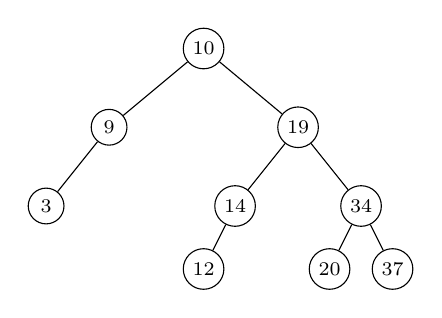
\begin{tikzpicture}[%level distance=5mm,
        level 1/.style={level distance=10mm,sibling distance=24mm},
        level 2/.style={level distance=10mm,sibling distance=16mm},
        level 3/.style={level distance=8mm,sibling distance=8mm},
        level 4/.style={level distance=6mm,sibling distance=6mm},
        font=\scriptsize,inner sep=2pt,every node/.style={draw,circle,minimum size=3ex}]

    \node {10}
    child   {node {9}
            child   {node {3}}
            child [missing]}
    child   {node {19}
            child  {node {14}
                    child   {node {12}}
                    child   [missing]}
            child   {node {34}
                    child {node {20}}
                    child   {node {37}}}};
\end{tikzpicture}






% \paragraph{Step 3: Insert 12 \\}
% \begin{tikzpicture}[%level distance=5mm,
%         level 1/.style={level distance=10mm,sibling distance=24mm},
%         level 2/.style={level distance=10mm,sibling distance=16mm},
%         level 3/.style={level distance=10mm,sibling distance=16mm},
%         font=\scriptsize,inner sep=2pt,every node/.style={draw,circle,minimum size=3ex}]

%     \node {9}
%     child [missing] % left child
%     child   {node {10} % right child
%             child [missing] % level 2
%             child   {node {12}}};
% \end{tikzpicture}

% \paragraph{Step 4: Insert 14 \\}
% \begin{tikzpicture}[%level distance=5mm,
%         level 1/.style={level distance=10mm,sibling distance=24mm},
%         level 2/.style={level distance=10mm,sibling distance=16mm},
%         level 3/.style={level distance=10mm,sibling distance=16mm},
%         font=\scriptsize,inner sep=2pt,every node/.style={draw,circle,minimum size=3ex}]

%     \node {9}
%     child [missing] % left child
%     child   {node {10} % right child
%             child [missing] % level 2
%             child   {node {12} % level 2
%                     child [missing] % level 3
%                     child   {node {14}}}};
% \end{tikzpicture}

% \paragraph{Step 5: Insert 3 \\}
% \begin{tikzpicture}[%level distance=5mm,
%         level 1/.style={level distance=10mm,sibling distance=24mm},
%         level 2/.style={level distance=10mm,sibling distance=16mm},
%         level 3/.style={level distance=10mm,sibling distance=12mm},
%         font=\scriptsize,inner sep=2pt,every node/.style={draw,circle,minimum size=3ex}]

%     \node {9}
%     child   {node {3} % left child
%         }
%     child   {node {10} % right child
%             child [missing] % level 2
%             child   {node {12} % level 2
%                     child [missing] % level 3
%                     child   {node {14}}}};
% \end{tikzpicture}

% \paragraph{Step 6: Insert 34 \\}
% \begin{tikzpicture}[%level distance=5mm,
%         level 1/.style={level distance=10mm,sibling distance=24mm},
%         level 2/.style={level distance=10mm,sibling distance=16mm},
%         level 3/.style={level distance=10mm,sibling distance=12mm},
%         level 4/.style={level distance=10mm,sibling distance=8mm},
%         font=\scriptsize,inner sep=2pt,every node/.style={draw,circle,minimum size=3ex}]

%     \node {9}
%     child   {node {3} % left child
%         }
%     child   {node {10} % right child
%             child [missing] % level 2
%             child   {node {12} % level 2
%                     child [missing] % level 3
%                     child   {node {14} % level 3
%                             child [missing] % level 4
%                             child   {node {34}}}}};
% \end{tikzpicture}

% \paragraph{Step 7: Insert 19 \\}
% \begin{tikzpicture}[%level distance=5mm,
%         level 1/.style={level distance=10mm,sibling distance=24mm},
%         level 2/.style={level distance=10mm,sibling distance=16mm},
%         level 3/.style={level distance=10mm,sibling distance=12mm},
%         level 4/.style={level distance=10mm,sibling distance=8mm},
%         level 5/.style={level distance=8mm,sibling distance=6mm},
%         font=\scriptsize,inner sep=2pt,every node/.style={draw,circle,minimum size=3ex}]

%     \node {9}
%     child   {node {3} % left child
%         }
%     child   {node {10} % right child
%             child [missing] % level 2
%             child   {node {12} % level 2
%                     child [missing] % level 3
%                     child   {node {14} % level 3
%                             child [missing] % level 4
%                             child   {node {34} % level 4
%                                     child   {node {19}} % level 5
%                                     child   [missing]}}}};
% \end{tikzpicture}

% \paragraph{Step 8: Insert 37 \\}
% \begin{tikzpicture}[%level distance=5mm,
%         level 1/.style={level distance=10mm,sibling distance=24mm},
%         level 2/.style={level distance=10mm,sibling distance=16mm},
%         level 3/.style={level distance=10mm,sibling distance=12mm},
%         level 4/.style={level distance=10mm,sibling distance=8mm},
%         level 5/.style={level distance=8mm,sibling distance=6mm},
%         font=\scriptsize,inner sep=2pt,every node/.style={draw,circle,minimum size=3ex}]

%     \node {9}
%     child   {node {3} % left child
%         }
%     child   {node {10} % right child
%             child [missing] % level 2
%             child   {node {12} % level 2
%                     child [missing] % level 3
%                     child   {node {14} % level 3
%                             child [missing] % level 4
%                             child   {node {34} % level 4
%                                     child   {node {19}} % level 5
%                                     child   {node {37}}}}}};
% \end{tikzpicture}

% \paragraph{Step 9: Insert 20 \\}
% \begin{tikzpicture}[%level distance=5mm,
%         level 1/.style={level distance=10mm,sibling distance=24mm},
%         level 2/.style={level distance=10mm,sibling distance=16mm},
%         level 3/.style={level distance=10mm,sibling distance=12mm},
%         level 4/.style={level distance=10mm,sibling distance=8mm},
%         level 5/.style={level distance=8mm,sibling distance=6mm},
%         level 6/.style={level distance=8mm,sibling distance=6mm},
%         font=\scriptsize,inner sep=2pt,every node/.style={draw,circle,minimum size=3ex}]

%     \node {9}
%     child   {node {3} % left child
%         }
%     child   {node {10} % right child
%             child [missing] % level 2
%             child   {node {12} % level 2
%                     child [missing] % level 3
%                     child   {node {14} % level 3
%                             child [missing] % level 4
%                             child   {node {34} % level 4
%                                     child   {node {19} % level 5
%                                             child [missing] % level 6
%                                             child  {node {20}}} % level 6
%                                     child   {node {37}}}}}};
% \end{tikzpicture}

$$ \blacksquare $$

\newpage

% Q2-b-1
\section*{Q2-b-1}

\text{Q: }
\paragraph{On the tree shown below, show each step of deleting the keys p, d, h. \\}
\text{\newline}
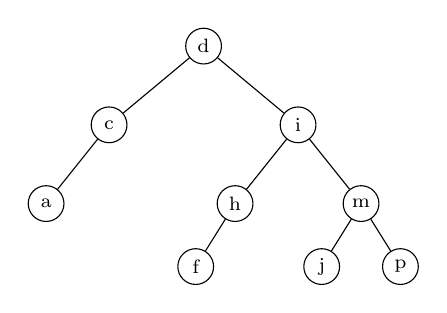
\begin{tikzpicture}[
        level 1/.style={level distance=10mm,sibling distance=24mm},
        level 2/.style={level distance=10mm,sibling distance=16mm},
        level 3/.style={level distance=8mm,sibling distance=10mm},
        font=\scriptsize,inner sep=2pt,every node/.style={draw,circle,minimum size=3ex}]

    \node{d}
    child   {
            node{c}
            child   {node{a}}
            child   [missing]
        }
    child   {
            node{i}
            child   {
                    node{h}
                    child   {node{f}}
                    child   [missing]
                }
            child{
                    node{m}
                    child   {node{j}}
                    child   {node{p}}
                }
        };

\end{tikzpicture}

\paragraph*{Step 1: Delete p \\}
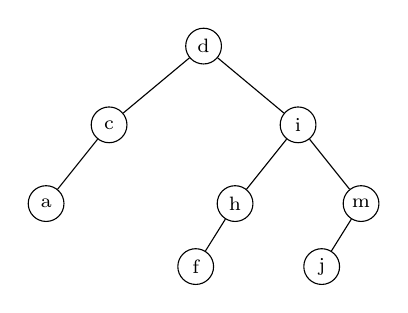
\begin{tikzpicture}[
        level 1/.style={level distance=10mm,sibling distance=24mm},
        level 2/.style={level distance=10mm,sibling distance=16mm},
        level 3/.style={level distance=8mm,sibling distance=10mm},
        font=\scriptsize,inner sep=2pt,every node/.style={draw,circle,minimum size=3ex}]

    \node{d}
    child   {
            node{c}
            child   {node{a}}
            child   [missing]
        }
    child   {
            node{i}
            child   {
                    node{h}
                    child   {node{f}}
                    child   [missing]
                }
            child{
                    node{m}
                    child   {node{j}}
                    child   [missing]
                }
        };
\end{tikzpicture}
$$ \blacksquare $$
\newpage

% Q2-b-2
\section*{Q2-b-2}
\text{Q: }
\paragraph*{On the tree shown below, show each step of deleting the keys p, d, h. \\}
\text{\newline}
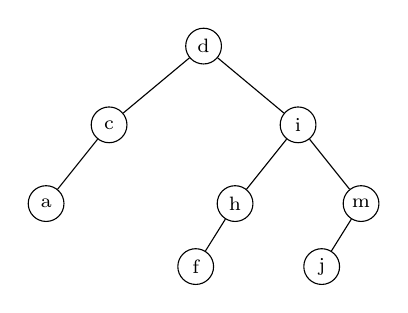
\begin{tikzpicture}[
        level 1/.style={level distance=10mm,sibling distance=24mm},
        level 2/.style={level distance=10mm,sibling distance=16mm},
        level 3/.style={level distance=8mm,sibling distance=10mm},
        font=\scriptsize,inner sep=2pt,every node/.style={draw,circle,minimum size=3ex}]

    \node{d}
    child   {
            node{c}
            child   {node{a}}
            child   [missing]
        }
    child   {
            node{i}
            child   {
                    node{h}
                    child   {node{f}}
                    child   [missing]
                }
            child{
                    node{m}
                    child   {node{j}}
                    child   [missing]
                }
        };
\end{tikzpicture}

\paragraph{Step 2: Delete d \\}

\text{1. Find the successor of d: \\}

Which is the leftmost node in the right subtree of d, which is f.\\

\text{2. Replace d with f}

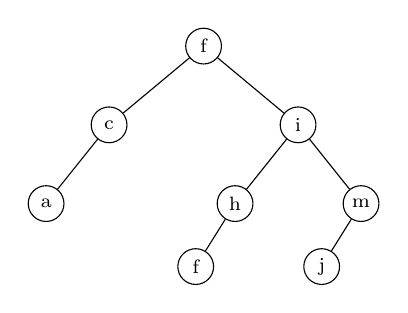
\begin{tikzpicture}[
        level 1/.style={level distance=10mm,sibling distance=24mm},
        level 2/.style={level distance=10mm,sibling distance=16mm},
        level 3/.style={level distance=8mm,sibling distance=10mm},
        font=\scriptsize,inner sep=2pt,every node/.style={draw,circle,minimum size=3ex}]

    \node{f}
    child   {
            node{c}
            child   {node{a}}
            child   [missing]
        }
    child   {
            node{i}
            child   {
                    node{h}
                    child   {node{f}}
                    child   [missing]
                }
            child{
                    node{m}
                    child   {node{j}}
                    child   [missing]
                }
        };
\end{tikzpicture}

\text{3. Delete f}

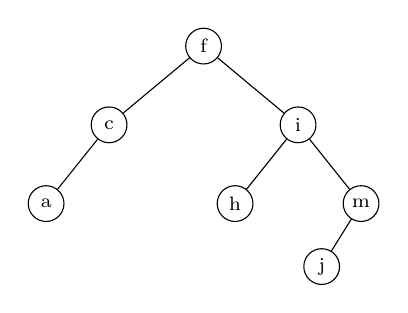
\begin{tikzpicture}[
        level 1/.style={level distance=10mm,sibling distance=24mm},
        level 2/.style={level distance=10mm,sibling distance=16mm},
        level 3/.style={level distance=8mm,sibling distance=10mm},
        font=\scriptsize,inner sep=2pt,every node/.style={draw,circle,minimum size=3ex}]

    \node{f}
    child   {
            node{c}
            child   {node{a}}
            child   [missing]
        }
    child   {
            node{i}
            child   {node{h}}
            child{
                    node{m}
                    child   {node{j}}
                    child   [missing]
                }
        };
\end{tikzpicture}

\vfill{$$\blacksquare$$}
\newpage

% Q2-b-3
\section*{Q2-b-3}
\text{Q: }
\paragraph*{On the tree shown below, show each step of deleting the keys p, d, h. \\}
\text{\newline}
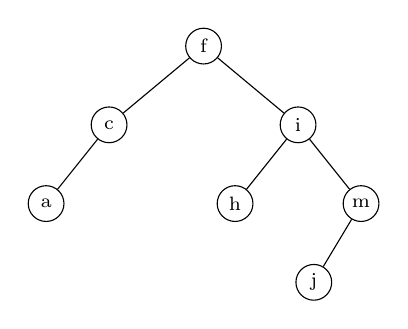
\begin{tikzpicture}[
        level 1/.style={level distance=10mm,sibling distance=24mm},
        level 2/.style={level distance=10mm,sibling distance=16mm},
        level 3/.style={level distance=10mm,sibling distance=12mm},
        level 4/.style={level distance=10mm,sibling distance=8mm},
        font=\scriptsize,inner sep=2pt,every node/.style={draw,circle,minimum size=3ex}]

    \node{f}
    child   {
            node{c}
            child   {node{a}}
            child   [missing]
        }
    child   {
            node{i}
            child   {node{h}}
            child{
                    node{m}
                    child   {node{j}}
                    child   [missing]
                }
        };
\end{tikzpicture}
\paragraph*{Step 3: Delete h \\}
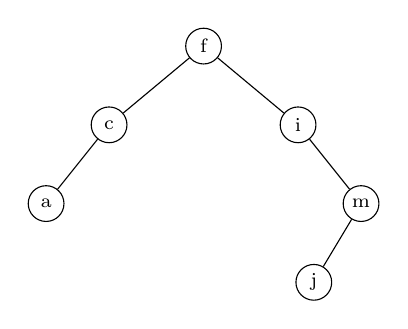
\begin{tikzpicture}[
        level 1/.style={level distance=10mm,sibling distance=24mm},
        level 2/.style={level distance=10mm,sibling distance=16mm},
        level 3/.style={level distance=10mm,sibling distance=12mm},
        level 4/.style={level distance=10mm,sibling distance=8mm},
        font=\scriptsize,inner sep=2pt,every node/.style={draw,circle,minimum size=3ex}]

    \node{f}
    child   {
            node{c}
            child   {node{a}}
            child   [missing]
        }
    child   {
            node{i}
            child   [missing]
            child{
                    node{m}
                    child   {node{j}}
                    child   [missing]
                }
        };
\end{tikzpicture}
\\
Imbalanced. Right heavy at node i. \\
Need a left rotation. \\
Left rotation: \\\\
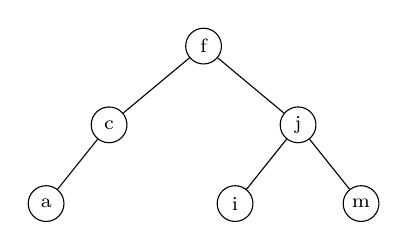
\begin{tikzpicture}[
        level 1/.style={level distance=10mm,sibling distance=24mm},
        level 2/.style={level distance=10mm,sibling distance=16mm},
        level 3/.style={level distance=10mm,sibling distance=12mm},
        level 4/.style={level distance=10mm,sibling distance=8mm},
        font=\scriptsize,inner sep=2pt,every node/.style={draw,circle,minimum size=3ex}]

    \node{f}
    child   {
            node{c}
            child   {node{a}}
            child   [missing]
        }
    child   {
            node{j}
            child   {node{i}}
            child   {node{m}}
        };
\end{tikzpicture}
$$ \blacksquare $$
\newpage

% Q2-c
\section*{Q2-c}
\text{Q: }
\paragraph*{Carefully consider the tree below. \\}
\text{\newline}
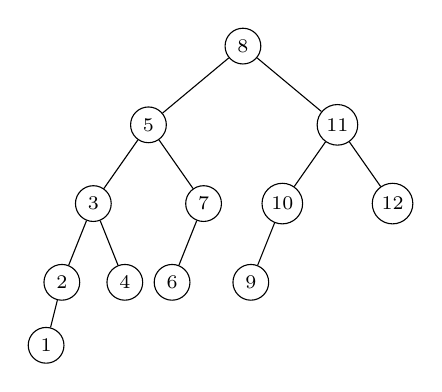
\begin{tikzpicture}[
        level 1/.style={level distance=10mm,sibling distance=24mm},
        level 2/.style={level distance=10mm,sibling distance=14 mm},
        level 3/.style={level distance=10mm,sibling distance=8mm},
        level 4/.style={level distance=8mm,sibling distance=4mm},
        font=\scriptsize,inner sep=2pt,every node/.style={draw,circle,minimum size=3ex}]

    \node{8}
    child   {
            node{5}
            child   {
                    node{3}
                    child   {node{2}
                            child {node{1}}
                            child [missing]
                        }
                    child   {node{4}}
                }
            child   {node{7}
                    child   {node{6}}
                    child   [missing]
                }
        }
    child   {
            node{11}
            child   {
                    node{10}
                    child   {node{9}}
                    child   [missing]
                }
            child{node{12}}
        };
\end{tikzpicture}

\begin{itemize}
    \item [-] If we start with an empty AVL tree, what sequence of insertions would result in this tree?
    \item [-] Show each step of deleting key 11.
\end{itemize}

\paragraph*{1. Insertion Sequence: (one possible sequence)}
\begin{itemize}
    \item Insert 8
    \item Insert 5
    \item Insert 11
    \item Insert 3
    \item Insert 7
    \item Insert 10
    \item Insert 12
    \item Insert 2
    \item Insert 4
    \item Insert 6
    \item Insert 9
    \item Insert 1
\end{itemize}
The only constraint is the key 1 must be inserted last. $ \blacksquare $
\newpage

\paragraph{2. Delete key 11:}
\subparagraph{Step 1: Find the seccessor of 11. \\}
\text{The leftmost node in the right subtree of root, i.e. 9.}

\subparagraph{Step 2: Replace 11 with 9. \\}
\text{Replace 11 with 9:}

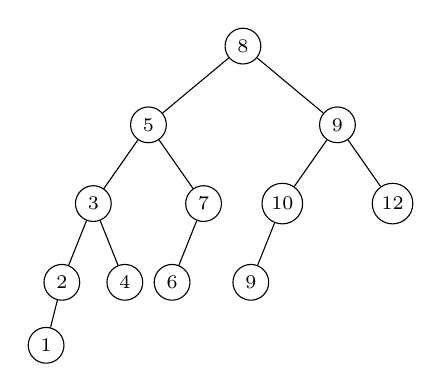
\begin{tikzpicture}[
        level 1/.style={level distance=10mm,sibling distance=24mm},
        level 2/.style={level distance=10mm,sibling distance=14 mm},
        level 3/.style={level distance=10mm,sibling distance=8mm},
        level 4/.style={level distance=8mm,sibling distance=4mm},
        font=\scriptsize,inner sep=2pt,every node/.style={draw,circle,minimum size=3ex}]

    \node{8}
    child   {
            node{5}
            child   {
                    node{3}
                    child   {node{2}
                            child {node{1}}
                            child [missing]
                        }
                    child   {node{4}}
                }
            child   {node{7}
                    child   {node{6}}
                    child   [missing]
                }
        }
    child   {
            node{9}
            child   {
                    node{10}
                    child   {node{9}}
                    child   [missing]
                }
            child{node{12}}
        };
\end{tikzpicture}

\subparagraph{Step 3: Delete 9. \\}
\text{Delete 9:}

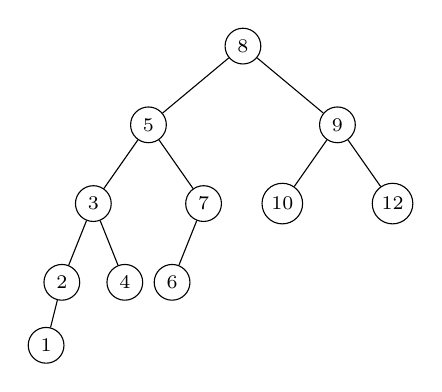
\begin{tikzpicture}[
        level 1/.style={level distance=10mm,sibling distance=24mm},
        level 2/.style={level distance=10mm,sibling distance=14 mm},
        level 3/.style={level distance=10mm,sibling distance=8mm},
        level 4/.style={level distance=8mm,sibling distance=4mm},
        font=\scriptsize,inner sep=2pt,every node/.style={draw,circle,minimum size=3ex}]

    \node{8}
    child   {
            node{5}
            child   {
                    node{3}
                    child   {node{2}
                            child {node{1}}
                            child [missing]
                        }
                    child   {node{4}}
                }
            child   {node{7}
                    child   {node{6}}
                    child   [missing]
                }
        }
    child   {
            node{9}
            child   {
                    node{10}
                    child   [missing]
                    child   [missing]
                }
            child{node{12}}
        };
\end{tikzpicture}
\\
Imbalanced. Left heavy at node 8. \\
Need a right rotation. \\
Right rotation: \\
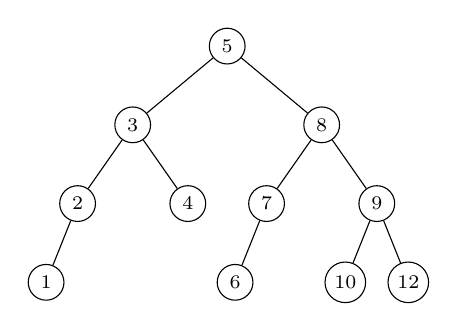
\begin{tikzpicture}[
        level 1/.style={level distance=10mm,sibling distance=24mm},
        level 2/.style={level distance=10mm,sibling distance=14 mm},
        level 3/.style={level distance=10mm,sibling distance=8mm},
        level 4/.style={level distance=8mm,sibling distance=4mm},
        font=\scriptsize,inner sep=2pt,every node/.style={draw,circle,minimum size=3ex}]

    \node{5}
    child   {
            node{3}
            child   {node{2}
                    child {node{1}}
                    child [missing]
                }
            child   {node{4}}
        }
    child   {node{8}
            child   {node{7}
                    child   {node{6}}
                    child   [missing]
                }
            child   {node{9}
                    child   {
                            node{10}
                            child   [missing]
                            child   [missing]
                        }
                    child{node{12}}
                }
        };
\end{tikzpicture}
$$ \blacksquare $$

\newpage

% Q4
\section*{Q4}
\text{Q: }
\text{Consider an ADT consisting of a set S of distinct integers and the following operations: \\}

\begin{itemize}
    \item search(S, x): Return true if x is in S and false otherwise.
    \item insert(S, x): Insert the element x into the set S.
          This operation has no effect if x is already in S.
    \item \text{delete(S, x): Delete the element x from the set S. This operation has no effect if x is not in S.}
    \item min\_difference(S): Given a set S with size of at least 2, return a pair of distinct integers (x, y),
          \newline
          with x $\in$ S, y $\in$ S, with the minimum absolute difference, i.e.
          \newline
          $\forall x', \forall y', (x' \neq y' \rightarrow |x - y| \leq |x' - y'|)$
\end{itemize}
\paragraph{}
Your task is to design a data structure to implement this ADT, \\
such that all operations are performed in $\mathcal{O} (\log\ n)$ time, \\
where $n = |S|$. You will do so by augmenting our familiar AVL tree.

\begin{enumerate}
    \item Describe all information that will be stored in the nodes.
    \item Provide pseudo-code for each required operation.
    \item Justify why your algorithms are correct and why they achieve the required time bound.
\end{enumerate}

\newpage

% \section*{An Evil Desing}
% \paragraph*{1. Describe all information that will be stored in the nodes. \\}
% \text{Given: A set S of distinct integers.}
% \newline
% \text{Also, the number of input must be finite. (In practical)}
% \newline
% \text{Also, we only discuss the time complexity, not the space complexity.}
% \newline
% \text{Then we come up with an evil design:}
% \newline
% \text{Say we have a bound for the value of the input, then we create a boolean array of size $n$}
% \paragraph{we put each input into the array, and use True to represent the input is in the set, False to represent the input is not in the set, and we use the value of the input as the index of the array.}
% \paragraph{Then it follows that the search, insert, and delete are all $\mathcal{O}(1)$}


% \paragraph*{1. Describe all information that will be stored in the nodes. (here the nodes is the elements of the array $S$)}
% \begin{itemize}
%     \item boolean is\_in\_set;
%     \item void *data;
% \end{itemize}
% \text{Extra information stored in a stack $T$:}
% \begin{itemize}
%     \item int min\_diff;
%     \item int index\_x;
%     \item int index\_y;
% \end{itemize}

% \paragraph*{2. Provide pseudo-code for each required operation.}
% \begin{itemize}
%     \item search(S, x): Return true if x is in S and false otherwise.
%     \begin{lstlisting}
%         return S[x]; // O(1)
%     \end{lstlisting}

%     \item insert(S, x): Insert the element x into the set S.
%           This operation has no effect if x is already in S.
%     \begin{lstlisting}
%         S[x] = True;
%         int pos_l = x;
%         int pos_r = x;

%         while (S[--pos_l] == False); // O(1), constant
%         while (S[++pos_r] == False); // O(1), constant
%         int diff_l = x - pos_l;
%         int diff_r = pos_r - x;

%         int diff = MIN(diff_l, diff_r);
%         int pos = (diff_l < diff_r) ? pos_l : pos_r;

%         if (diff < T.top.min_diff) {
%             T.push(diff, pos, x);
%         }

%     \end{lstlisting}

%     \item \text{delete(S, x): Delete the element x from the set S. This operation has no effect if x is not in S.}
%     \begin{lstlisting}
%         S[x] = False;

%         if (T.top.index_x == x) {
%             T.pop();
%         }
%         else if (T.top.index_y == x) {
%             T.pop();
%         }
%         else {
%             list = T.find(x);
%             for i in list:
%                 T.
%                 // Bad design, must exceed the time complexity
%         }


%     \end{lstlisting}

%     \item min\_difference(S): Given a set S with size of at least 2, return a pair of distinct integers (x, y),
%           \newline
%           with x $\in$ S, y $\in$ S, with the minimum absolute difference, i.e.
%           \newline
%           $\forall x', \forall y', (x' \neq y' \rightarrow |x - y| \leq |x' - y'|)$
%     \begin{lstlisting}
%         return T.top.min_diff;
%     \end{lstlisting}
% \end{itemize}

% $$ \blacksquare $$
% \newpage

\section*{Augmented AVL Tree}
\paragraph*{1. Describe all information that will be stored in the nodes.}
\begin{itemize}
    \item int key;
    \item void *data;
    \item int height;
    \item node *left;
    \item node *right;
    \item int relative\_min\_diff; // augmented information
    \item tuple (x, y) min\_pair; // augmented information
          % \item node *parent; // augmented information
\end{itemize}

*Note that here 2 augmented information are introduced:

\begin{itemize}
    \item relative\_min\_diff: the min difference in the subtree at the node.
    \item min\_pair: the pair of integers with the minimum difference in the subtree at the node.
\end{itemize}

\newpage

\paragraph*{2. Provide pseudo-code for each required operation.}
\begin{itemize}
    \item search(S, x): Return true if x is in S and false otherwise.
          \begin{lstlisting}
        return BST_search(S, x);
        // Where BST_search is the search function of a BST
        // See below:
        def BST_search(S, x):
            if S == NULL:
                return False
            if x == S.key:
                return True
            else:
                if x < S.key:
                    return BST_search(S.left, x)
                else:
                    return BST_search(S.right, x)
    \end{lstlisting}

          \newpage

    \item insert(S, x): Insert the element x into the set S.
          This operation has no effect if x is already in S.
          \begin{lstlisting}
        def insert(S, x):
            if S == NULL:
                S = new node
                S.key = x
                S.left = NULL
                S.right = NULL
                return S
            if x == S.key:
                return S
            else:
                if x < S.key:
                    S.left = insert(S.left, x)
                else:
                    S.right = insert(S.right, x)
            
            update_height(S) // The same as AVL tree
            S = balance(S) // The same as AVL tree
            update_min_diff(S) // See helper functions below
            return S
    \end{lstlisting}

          \newpage

    \item delete(S, x): Delete the element x from the set S.
          This operation has no effect if x is not in S.
          \begin{lstlisting}
        def delete(S, x):
            if S == NULL:
                return S
            if x == S.key:
                if S.left == NULL and S.right == NULL:
                    return NULL
                if S.left == NULL:
                    return S.right
                if S.right == NULL:
                    return S.left
                else:
                    S.key = find_min(S.right)
                    S.right = delete(S.right, S.key)
            else:
                if x < S.key:
                    S.left = delete(S.left, x)
                else:
                    S.right = delete(S.right, x)
            
            update_height(S) // The same as AVL tree
            S = balance(S) // The same as AVL tree
            update_min_diff(S) // See helper functions below
            return S
    \end{lstlisting}

          \newpage

    \item min\_difference(S): Given a set S with size of at least 2, return a pair of distinct integers (x, y),
          \newline
          with x $\in$ S, y $\in$ S, with the minimum absolute difference, i.e.
          \newline
          $\forall x', \forall y', (x' \neq y' \rightarrow |x - y| \leq |x' - y'|)$
          \begin{lstlisting}
        def min_difference(S):
            return S.min_pair
    \end{lstlisting}
\end{itemize}

\paragraph*{Helper functions}

\begin{itemize}
    \item update\_height(S): Update the height of the node S.
          $ \mathcal{O}(1) $ time complexity.
          \begin{lstlisting}
        def height(S):
            if S == NULL:
                return -1
            else:
                return S.height

        def update_height(S):
            S.height = 1 + max(height(S.left), height(S.right))
    \end{lstlisting}

    \item balance(S): Balance the node S.
          $ \mathcal{O}(1) $ time complexity.
          \begin{lstlisting}
        def balance(S):
            if S == NULL:
                return S
            if height(S.left) - height(S.right) > 1:
                if height(S.left.left) >= height(S.left.right):
                    S = rotate_right(S)
                else:
                    S.left = rotate_left(S.left)
                    S = rotate_right(S)
            else if height(S.right) - height(S.left) > 1:
                if height(S.right.right) >= height(S.right.left):
                    S = rotate_left(S)
                else:
                    S.right = rotate_right(S.right)
                    S = rotate_left(S)
            return S
    \end{lstlisting}

    \item update\_min\_diff(S): Update the augmented information of the node S.

          $ \mathcal{O}(1) $ time complexity.
          \begin{lstlisting}
        def update_min_diff(S):
            if S == NULL:
                return
            if S.left == NULL and S.right == NULL:
                S.relative_min_diff = MAX_INT
// It it more understandable to use 0 since the difference is always positive.
// But we need to use MAX_INT for the ease of implementation.
// Actually, `if S.left.relative_min_diff <= S.right.relative_min_diff:'
                S.min_pair = (NULL, NULL)
                return
            if S.left == NULL:
                S.relative_min_diff = S.right.relative_min_diff
                S.min_pair = S.right.min_pair
                return
            if S.right == NULL:
                S.relative_min_diff = S.left.relative_min_diff
                S.min_pair = S.left.min_pair
                return
            
            if S.left.relative_min_diff <= S.right.relative_min_diff:
                S.relative_min_diff = S.left.relative_min_diff
                S.min_pair = S.left.min_pair
            else:
                S.relative_min_diff = S.right.relative_min_diff
                S.min_pair = S.right.min_pair
            
            return S
    \end{lstlisting}
\end{itemize}

$$ \blacksquare $$
\newpage

\paragraph*{3. Justify why your algorithms are correct and why they achieve the required time bound.}

\section*{Proof of correctness}

\begin{itemize}
    \item search(S, x): The search function of a AVL is correct,
          and the introduced helper function `update\_min\_diff()' does not change the correctness of the search function.
    \item insert(S, x): The insert function of a AVL is correct,
          and the introduced helper function `update\_min\_diff()' are correct.
    \item delete(S, x): The delete function of a AVL is correct,
          and the introduced helper function `update\_min\_diff()' are correct.
    \item min\_difference(S): It basically returns a value stored in the input node.
          To prove the correctness of this function, we need to prove that the value stored in the input node is correct,
          which will be proved in the proof of the `update\_min\_diff()' function.
    \item update\_min\_diff(S): The correctness of this function is based on the following two facts:
          \begin{enumerate}
              \item $\left[Base\ Case\right]$ If the node S is a leaf node, then the value stored in S is correct.
                    \begin{itemize}
                        \item The value stored in S is the minimum absolute difference of the set S,
                              where the set S is a set with only one element, so the minimum absolute difference of the set S is
                              a special case of the minimum absolute difference of a set, which is defined as $MAX\_INT$
                              (because the real minimum absolute difference is always greater than $MAX\_INT$ in a set of distinct integers).
                        \item Therefore, the value stored in S is correct.
                    \end{itemize}

              \item  $\left[I.H.\right]$ The value stored in the node S is correct.

              \item $\left[I.S.\right]$ Prove: the value stored in the parent node of S is correct. \\
                    Let S' be the parent node of S, and let S\_L and S\_R be the left child and right child of S' respectively.
                    \begin{itemize}
                        \item The value of S\_L.relative\_min\_diff is the minimum absolute difference of the set S\_L.
                        \item The value of S\_R.relative\_min\_diff is the minimum absolute difference of the set S\_R.
                        \item The value of S'.relative\_min\_diff is the minimum of S\_L.relative\_min\_diff and S\_R.relative\_min\_diff.
                        \item $\Rightarrow$ The value of S'.relative\_min\_diff is the minimum absolute difference of both subset S\_L and S\_R.
                        \item $\Rightarrow$ The value of S'.relative\_min\_diff is the minimum absolute difference of the set S'.
                        \item $\Rightarrow$ The value of S'.relative\_min\_diff is correct.
                    \end{itemize}
          \end{enumerate}
\end{itemize}
$$ \blacksquare $$

\section*{Proof of time complexity}

\begin{itemize}
    \item search(S, x): O(log n) because the search function of a AVL is O(log n),
          and the introduced helper functions are O(1).
    \item insert(S, x): O(log n) because the insert function of a AVL is O(log n),
          and the introduced helper functions are O(1).
    \item delete(S, x): O(log n) because the delete function of a AVL is O(log n),
          and the introduced helper functions are O(1).
    \item min\_difference(S): O(1) because it basically returns a value stored in the input node.
\end{itemize}
Above are the time complexities of the four functions, which are all within O(log n).
$$ \blacksquare $$



% \mbox{}
% \vfill{$$\blacksquare$$}
\end{document}